\documentclass[12pt]{article}
\usepackage{pslatex} % Font Times New Roman

\usepackage{amsmath,amssymb,amsfonts,amsthm,fancyhdr,lastpage}
\usepackage{makeidx, graphicx, mdwlist, listings}

\setlength{\textheight}{9.0in}
\setlength{\topmargin}{-.5in}
\setlength{\textwidth}{6.5in}
\setlength{\oddsidemargin}{-.0in}
\setlength{\parskip}{6pt}


\renewcommand{\headrulewidth}{0pt}
\setlength{\headsep}{.35in}
\addtolength{\headheight}{2.5pt} 

\usepackage{graphicx}

\begin{document}

\title{Comparative Analysis of Methods for Obtaining Realistic Graphs from Kekule Cells}
\author{Aaron Germuth and Alex Aravind \\\\  
Department of Computer Science \\
University of Northern British Columbia \\
E-mail: (germuth,csalex)@unbc.ca}
\maketitle

\section{Realistic Graphs}

Hesselink presented a complete classification for the switching behaviour seen in conjugated molecules \cite{H13}. He formulated a recursive method for obtaining graphs for each Kekule cell or classification. Each graph was a model for a conjugated carbon molecule, where nodes are atoms, and edges are bonds. However, Hesselink made no attempt to create graphs that can be mapped to realistic molecules. We define a realistic graph as one that can be directly mapped to the actual physical molecule it is trying to represent (see Figure ~\ref{fig:graphToMolecule}). 

\begin{figure}[ht!]
\centering
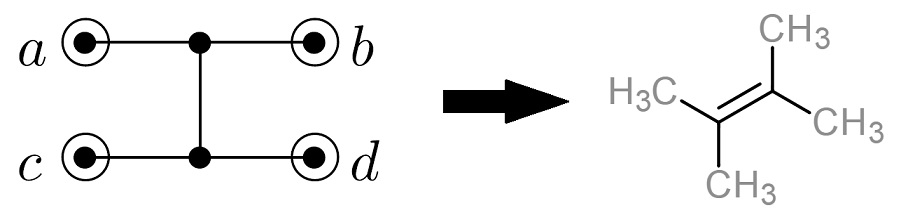
\includegraphics[width=110mm]{graphToMolecule.jpg}
\label{fig:graphToMolecule}
\end{figure}

This means the graph must meet the restrictions of carbon chemistry. We are dealing with a small subset of carbon chemistry, specifically polycyclic aromatic hydrocarbons. In order to verify whether a graph is realistic, we ensure the following restrictions:

\begin{enumerate*}
  \item All nodes have a degree of at most 3.
  \item All ports have a degree of at most 2.
  \item All cycles are of size 5 or 6
  \item All attached cycles are connected by precisely 2 atoms.
  \item Certain arrangements of specific ring complexes are prohibited
  \item The graph must be connected
  \item The graph must have a Kekule Cell matching the desired switching behaviour
\end{enumerate*}

These restrictions prevent the large majority of unrealistic graphs. Our restrictions make no attempt to ensure all graphs can be synthesized. 

\section{Graph Modification}

Many graphs end up satisfying most of the above restrictions except for one. In such cases, it is often feasible to modify the graph to alleviate that specific restriction. Nodes of high degree can often be split into multiple nodes of lower degree using a merge procedure in reverse, outline by Hesselink et al\cite{HH13}. 

Cycles can often be extended or shortened, two nodes at a time to meet the cycle size restriction (see Figure ~\ref{fig:cycleExtension}). This has no effect on the Kekul\'e cell. This procedure is nearly identical to operation v of \cite{v06}. Care must be taken to not select two nodes which also are a part of another cycle, as the resulting graph will contain unrealistic bonding distances and cycle connectivity. The opposite procedure can be used to contract cycles.

\begin{figure}[ht!]
\centering
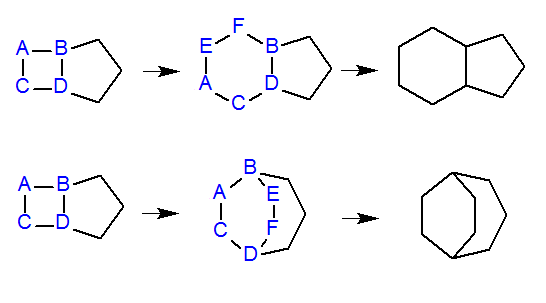
\includegraphics[width=90mm]{cycleExtension.png}
\caption{This shows the extension of the left 4 cycle into a proper 6 cycle. The top half shows a correct procedure, selecting to add nodes between A and B. The bottom half shows the incorrect procedure of adding two nodes in between B and D. Double bonds are excluded from this diagram for clarity.}
\label{fig:cycleExtension}
\end{figure}

Disjoint graphs can often be connected using the following procedure. Internal verticies are added which always conjugate ’within’ themselves, and therefore do not interfere with the cell (see Figure ~\ref{fig:disjoint}).

\begin{figure}[ht!]
\centering
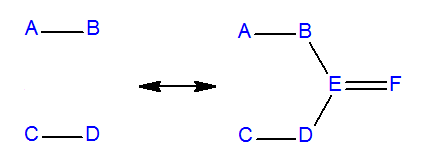
\includegraphics[width=90mm]{disjoint2.png}
\caption{Procedure used to connect a disjoint graph while preserving the Kekule cell. Two new nodes E and F can be added which must form a double bond in every resonance structure. Therefore the behaviour of B and D is unaffected.This procedure is similar to Operation iii and vi of [3]. }
\label{fig:disjoint}
\end{figure}

\pagebreak

\section{Mapping from Kekul\'e Cell to Graph}

Given a graph, the cell can be calculated according to the procedure outlined in Section 4.1 of \cite{H13}. It begins by removing components from the graph and finding the cell of smaller and smaller sections. These results are eventually combined into the Kekul\'e Cell for the entire graph. We used 4 alternative methods to obtain graphs for each classification. All methods limit their graphs to a maximum of 30 nodes.

\subsection{Template Molecules}

Common polycyclic aromatic hydrocarbons were used as template molecules. All possible combinations of port placements are tested for their cell. Molecules used includes Benzene, Napthalene, Azulene, Acenaphthylene, Pyracylene, Biphenyl, Anthracene, Phenanthrene, and Pyrene.

\subsection{Genetic Algorithm}

A genetic algorithm is used to search for graphs which apply to a given cell. The algorithm begins by randomly generating a population of graphs. In each iteration, the survivors of last generation's population must be chosen. This is done by selecting the best performing graphs (fitness-wise), along with a smaller amount of random graphs. Random graphs are added to ensure genetic diversity in the population. This sub-population now undergoes genetic operations such as mutation and crossover. 

\subsubsection{Mutation}

Mutation involves randomly perturbing graphs to obtain new ones. Mutations include:
\begin{enumerate*}
\item Addition of a node
\item Removal of a random node, and all edges to it
\item Addition of a random edge \footnote{ Edges are randomly chosen until an edge is found that can be added without breaking our restrictions on the degree of vertices.}
\item Removal of a random edge
\item Port Extension
\end{enumerate*}

Port extension involves adding a new node in the position of every port, and then adding the port connected to that node. This is often useful for spreading the ports out and allowing new edges without breaking our degree restrictions. This is not guaranteed to preserve the Kekule Cell. See Figure ~\ref{fig:portExtension}.

\begin{figure}[ht!]
\centering
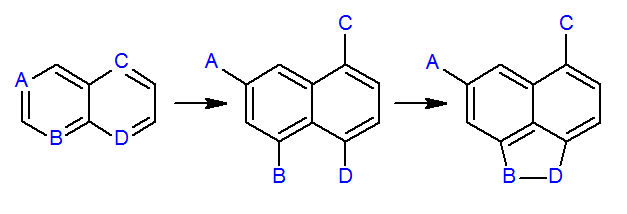
\includegraphics[width=110mm]{portExtension.png}
\caption{Napthalene (left) undergoing a port extension (center). Notice that after the port extension, it is now feasible to add an edge between B and D, which can then create Acenaphthene (right).}
\label{fig:portExtension}
\end{figure}

\subsubsection{Crossover}

Crossover begins by randomly selecting 2 graphs from the sub-population. These graphs are combined to create a new child graph. Children receive all edges which both parents share, and have a 50\% chance to get any other edge found in one of the parents. This creates children which are a hybrid of both their parents.

\subsubsection{Fitness Function}

Fitness values are integers given to a graph. Any graph's cell can be calculated using Hesselink's procedure \cite{H13}. The fitness is calculated by iterating over the graphs cell compared to the cell we are evolving towards. For every port assignment they share, the fitness is incremented by one. For every port assignment that is missing, or is extra, fitness is decremented one point. 

\subsection{Complexity}

The large running time of Hesselink's recursive procedure for determining the cell of a  graph is the bottleneck for most of our processes. Modification, random graphs, and template molecules return results immediately. However, in order for random graphs to reach the full potential, many iterations are needed, upwards of 100,000. The genetic algorithm is by far the slowest solution, in the worst case it can take over a hour to search for a single cell. The population size or generation number can be reduced however to sacrifice results for speed. The genetic algorithm also has the largest memory requirement, but since only the most recent population in saved in memory, it shouldn't take more than 750 MB with the default population size. 

\section{Results}

Our methods were able to discover realistic graphs as per the previous restrictions for all cells of rank 4 and 5. Hesselink was able to find graphs with no restrictions for 210 out of 214 cells with rank 6 \cite{H13}. None of our methods were able to find graphs, realistic or not, for the 4 missing cells of rank 6. We compare the performance of each of our methods based on cells of rank 6 (see Table 1).

Table 1. The amount of Kekule cells of rank 6 that each method was able to find realistic graphs for, according to our restrictions.
\begin{center}
  \begin{tabular}{ | l | r |}
    \hline
    Methodology & Cells of Rank 6 Found \\
    \hline
    Template Molecules & 44 \\
    Graph Modification & 32 \\
    Random Graphs & 135 \\
    Genetic Algorithm & 70 \\
    \hline
  \end{tabular}
\end{center}

It seems stochastic methods yield the best results for generating realistic graphs. As the cell number increases (K1 - K214), the graphs get more complex. In total we have found realistic graphs for 165 out of 214 graphs, with most of these clustering towards the beginning.

It would be interesting to see additional cell-invariant operations. Not only would this improve the raw modification method, but unrealistic graphs from other methods may also be able to be modified. It would also be interesting to discover to what extent this class of molecules is synthesizable. 

Polycylic aromatic hydrocarbons are commonly produced as byproducts of fuel burning, and have been classified as carcinogenic, mutagenic, and teratogenic. This could pose a challenge if we wish to use large aromatic hydrocarbons in circuitry. 

\begin{thebibliography}{abrv}

\bibitem{H13} W. H. Hesselink, Graph Theory for alternating hydrocarbons with attached ports. Indagationes Mathematicae, Elsevier, 24:115141, 2013.
\bibitem{HH13} W.H. Hesselink, J.C. Hummelen, H.T. Jonkman, H.G. Reker, G.R. Renardel de Lavalette, M.H. van der Veen, Kekule Cells for Molecular Computation. Cornell University Library Online, 2013.
\bibitem{v06} M.H. van der Veen. $\pi$-Logic. PhD thesis, University of Groningen, May 2006.
\bibitem{SMILES} Weininger, David. "SMILES, a chemical language and information system. 1. Introduction to methodology and encoding rules." Journal of chemical information and computer sciences 28.1 (1988): 31-36.
\bibitem{HK88} A.J. Heeger, S. Kivelson, J.R. Schrieffer, and W.-P Su. Solitons in conducting polymers, Rev. Mod. Phys.,60:781, 1988.
\bibitem{Moore} G. E. Moore, Cramming more components onto integrated circuits. Electronics Magazine. p. 4. Retrieved 2006-11-11. 
\bibitem{CDK} Steinbeck, Christoph, et al. "The Chemistry Development Kit (CDK): An open-source Java library for chemo-and bioinformatics." Journal of chemical information and computer sciences 43.2 (2003): 493-500.
\bibitem{MooreEnd} C. A. Mack, Fifty Years of Moore's Law. IEEE Transactions on semiconductor manufacturing, 24:2 2011.
\bibitem{OmniConj} M. H. van der Veen, M. T. Rispens, H. T. Jonkman, and J. C. Hummelen, Molecules with Linear $\pi$-Conjugated Pathways between all Substituents: Omniconjugation. Adv. Function Mater, 14:3, 2004.
\bibitem{openPath} S.N. Yalirahi, M.A. Ratner, Interplay of topology and chemical stability on the electronic transport of molecular junctions, Ann. New York Acad. Sci. 960 (2002) 153.
\bibitem{9} J. Reichert, R. Ochs, D. Beckmann, H. B. Weber, M. Mayor, H. von Löhneysen,Phys. Rev. Lett. 2002, 88, 176804. 
\bibitem{10} A. Aviram, M. A. Ratner, Chem. Phys. Lett. 1974, 29, 277.
\bibitem{11} D. B. Strukov, K. K. Likharev, Nanotechnology 2005, 16, 137.
\bibitem{12} Y. Karzazi, J. Cornil, J. L. Brédas, J. Am. Chem. Soc. 2001, 123, 10076.
\bibitem{13} J. M. Tour, M. Kozaki, J. M. Seminario, J. Am. Chem. Soc. 1998, 120, 8486.
\bibitem{14} A. Aviram, J. Am. Chem. Soc. 1988, 110, 5687.
\bibitem{15} H. W. Ch. Postma, T. Teepen, Z. Yao, M. Grifoni, C. Dekker, Science 2001, 293, 76.
\bibitem{16} C. Joachim, J. K. Gimzewski, Chem. Phys. Lett. 1997, 265, 353.
\bibitem{17} T. D. Anthopoulos, C. Tanase, S. Setayesh, E. J. Meijer, J. C. Hummelen, P. W. M. Blom, D. M. de Leeuw, Adv. Funct. Mater. 2004, 16, 2174.
\bibitem{18} G. M. Tsivgoulis, J.-M. Lehn, Chem. Eur. J. 1996, 2, 1399.
\bibitem{19} J. J. D. de Jong, L. N. Lucas, R. M. Kellogg, J. H. van Esch, B. L. Feringa, Science 2004, 304, 278.
\bibitem{20} A. P. de Silva, H. Q. N. Gunaratne, C. P. McCoy, Nature 1993, 364, 42.
\bibitem{21} F. M. Raymo, S. Giordani, J. Org. Chem. 2003, 68, 4158.
\bibitem{22} K. Rurack, A. Koval'chuck, J. L. Bricks, J. L. Slominskii, J. Am. Chem. Soc. 2001, 123, 6205.
\bibitem{23} D. Parker, J. A. G. Williams, Chem. Commun. 1998, 245.
\bibitem{24} A. P. de Silva, I. M. Dixon, H. Q. N. Gunaratne, T. Gunnlaugsson, P. R. S. Maxwell, T. E. Rice, J. Am. Chem. Soc. 1999, 121, 1393.

\bibitem{HuckelBad} Roberts, J. D., Streitwieser Jr, A., and Regan, C. M. Small-Ring Compounds. X. Molecular Orbital Calculations of Properties of Some Small-Ring Hydrocarbons and Free Radicals. Journal of the American Chemical Society, 74(18), 4579-4582. 1952.

\bibitem{HuckelExtension} Kruszewski, J., and Krygowski, T. M. An Extension of the Hückel 4N+ 2 Rule to Polycyclic Non-alternant Conjugated Hydrocarbons. Canadian Journal of Chemistry, 53(6), 945-951. 1975.

\bibitem{methylPentalene} Hafner, K., Donges, R., Goedecke, E. and 
Kaiser, R. Concerning Pentalene, 2-Methylpentalane, and 1,3-
Dimethylpentalene. Angew. Chem. Int. Ed. Engl., 12: 337-339. 1973.

\bibitem{nitrogenPentalene} Hafner, K., Bangert, K. F. and Orfanos, V 1,3-Bis(dimethylamino)pentalene. Angew. Chem. Int. Ed. Engl., 6: 451–452. 1967.

\end{thebibliography}

\end{document}
